在论文中,Geoffrey Hinton 介绍 Capsule 为:「Capsule 是一组神经元,其输入输出向量表示特定实体类型的实例化参数(即特定物体、概念实体等出现的概率与某些属性)。我们使用输入输出向量的长度表征实体存在的概率,向量的方向表示实例化参数(即实体的某些图形属性)。同一层级的 capsule 通过变换矩阵对更高级别的 capsule 的实例化参数进行预测。当多个预测一致时(本论文使用动态路由使预测一致),更高级别的 capsule 将变得活跃。」

Capsule 中的神经元的激活情况表示了图像中存在的特定实体的各种性质。这些性质可以包含很多种不同的参数,例如姿势(位置,大小,方向)、变形、速度、反射率,色彩、纹理等等。而输入输出向量的长度表示了某个实体出现的概率,所以它的值必须在 0 到 1 之间。

为了实现这种压缩,并完成 Capsule 层级的激活功能,Hinton 等人使用了一个被称为「squashing」的非线性函数。该非线性函数确保短向量的长度能够缩短到几乎等于零,而长向量的长度压缩到接近但不超过 1 的情况。以下是该非线性函数的表达式:
\begin{equation}\label{eq1:Squash}
\mathbf{v}_j=\frac{\|s_j\|^2}{1+\|s_j\|^2}\frac{s_j}{\|s_j\|}
\end{equation}

其中 $v_j$ 为 Capsule j 的输出向量,$s_j$ 为上一层所有 Capsule 输出到当前层 Capsule j 的向量加权和,简单说 $s_j$ 就为 Capsule j 的输入向量。该非线性函数可以分为两部分,即$\frac{\|s_j\|^2}{1+\|s_j\|^2}$和$\frac{s_j}{\|s_j\|}$
前一部分是输入向量 $s_j$ 的缩放尺度,第二部分是输入向量$s_j$ 的单位向量,该非线性函数既保留了输入向量的方向,又将输入向量的长度压缩到区间 [0,1) 内。$s_j$ 向量为零向量时$v_j$ 能取到 0,而 $s_j$ 无穷大时 $v_j$ 无限逼近 1。该非线性函数可以看作是对向量长度的一种压缩和重分配,因此也可以看作是一种输入向量后「激活」输出向量的方式。
 
 那么如上所述,Capsule 的输入向量就相当于经典神经网络神经元的标量输入,而该向量的计算就相当于两层 Capsule 间的传播与连接方式。输入向量的计算分为两个阶段,即线性组合和 Routing,这一过程可以用以下公式表示:]
\begin{equation}\label{eq2:Routing}
	s_j=\sum_{i}c_{ij}\hat{\mathbf{u}}_{j|u},\hat{\mathbf{u}}_{j|i}=\mathbf{W_{ij}}\mathbf{u}_i
\end{equation}
其中$\hat{u}_{j|i}$为$u_i$ 的线性组合,这一点可以看作是一般全连接网络前一层神经元以不同强弱的连接输出到后一层某个神经元。只不过 Capsule 相对于一般神经网络每个结点都有一组神经元(以生成向量),即 $\hat{u}_{j|i}$ 表示上一层第 i 个 Capsule 的输出向量和对应的权重向量相乘($W_{ij}$ 表示向量而不是元素)而得出的预测向量。$\hat{u}_{j|i}$ 也可以理解为在前一层为第 i 个 Capsule 的情况下连接到后一层第 j 个 Capsule 的强度。

在确定 $\hat{u}_{j|i}$ 后,我们需要使用 Routing 进行第二个阶段的分配以计算输出结点 $s_j$,这一过程就涉及到使用动态路由(dynamic routing)迭代地更新 $c_{ij}$。通过 Routing 就能获取下一层 Capsule 的输入 $s_j$,然后将 $s_j$ 投入「Squashing」非线性函数后就能得出下一层 Capsule 的输出。后面我们会重点解释 Routing 算法,但整个 Capsule 层及它们间传播的过程已经完成了。

所以整个层级间的传播与分配可以分为两个部分,第一部分是下图$ u_i$ 与 $\hat{u}_{j|i}$ 间的线性组合,第二部分是 $\hat{u}_{j|i}$ 与 $s_j$ 之间的 Routing 过程。若读者对传播过程仍然不是太明晰,那么可以看以下两层 Capsule 单元间的传播过程,该图是根据我们对传播过程的理解而绘制的:
\begin{figure}[H]
	\centering
	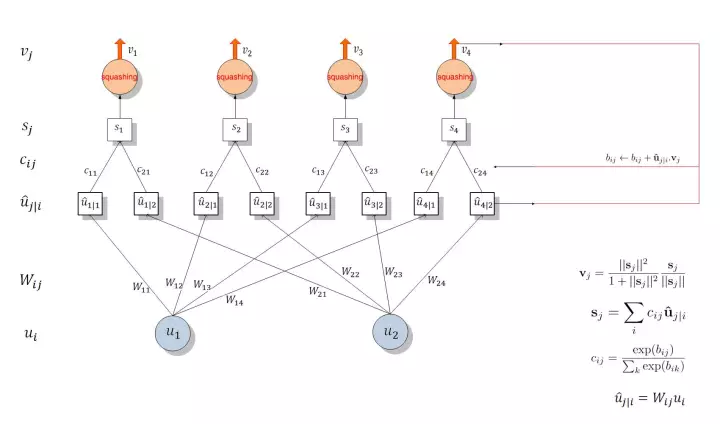
\includegraphics[scale=0.5]{capsule.png}
	\caption{capsule框架图}
	\label{fig:1}
\end{figure}
如上所示,该图展示了 Capsule 的层级结构与动态 Routing 的过程。最下面的层级 $u_i$ 共有两个 Capsule 单元,该层级传递到下一层级 $v_j$ 共有四个 Capsule。$u_1$ 和 $u_2$ 是一个向量,即含有一组神经元的 Capsule 单元,它们分别与不同的权重 $W_{ij}$(同样是向量)相乘得出 $\hat{u}_{j|i}$。例如 $u_1$ 与 $W_{12}$ 相乘得出预测向量 $\hat{u}_{2|1}$。随后该预测向量和对应的「耦合系数」$c_{ij}$ 相乘并传入特定的后一层 Capsule 单元。不同 Capsule 单元的输入 $s_j$ 是所有可能传入该单元的加权和,即所有可能传入的预测向量与耦合系数的乘积和。随后我们就得到了不同的输入向量 $s_j$,将该输入向量投入到「squashing」非线性函数就能得出后一层 Capsule 单元的输出向量 $v_j$。然后我们可以利用该输出向量 $v_j$ 和对应预测向量 $\hat{u}_{j|i}$ 的乘积更新耦合系数 $c_{ij}$,这样的迭代更新不需要应用反向传播。
\section{动态路由算法}
因为按照 Hinton 的思想,找到最好的处理路径就等价于正确处理了图像,所以在 Capsule 中加入 Routing 机制可以找到一组系数 $c_{ij}$,它们能令预测向量 $hat{u}_{j|i}$ 最符合输出向量 $v_j$,即最符合输出的输入向量,这样我们就找到了最好的路径。

按照原论文所述,$c_{ij}$ 为耦合系数(coupling coefficients),该系数由动态 Routing 过程迭代地更新与确定。Capsule i 和后一层级所有 Capsule 间的耦合系数和为 1,即图一 $c_{11}+c_{12}+c_{13}+c_{14}=1$。此外,该耦合系数由「routing softmax」决定,且 softmax 函数中的 logits $b_{ij}$ 初始化为 0,耦合系数 $c_{ij}$ 的 softmax 计算方式为:
\begin{equation}
	c_{ij}=\frac{exp(b_{ij})}{\sum_{k}exp(b_{ik})}
\end{equation}
$b_{ij}$ 依赖于两个 Capsule 的位置与类型,但不依赖于当前的输入图像。我们可以通过测量后面层级中每一个 Capsule j 的当前输出 $v_j$ 和 前面层级 Capsule i 的预测向量间的一致性,然后借助该测量的一致性迭代地更新耦合系数。本论文简单地通过内积度量这种一致性,即 ,这一部分也就涉及到使用 Routing 更新耦合系数。

Routing 过程就是上图\ref{fig:1} 右边表述的更新过程,我们会计算 $v_j$ 与 $\hat{u_{i|j}}$ 的乘积并将它与原来的 $b_{ij}$ 相加而更新 $b_{ij}$,然后利用 $softmax(b_{ij})$ 更新 $c_{ij}$ 而进一步修正了后一层的 Capsule 输入 $s_j$。当输出新的 $v_j$ 后又可以迭代地更新 $c_ij$,这样我们不需要反向传播而直接通过计算输入与输出的一致性更新参数。

该 Routing 算法更具体的更新过程可以查看以下伪代码:
%\begin{table}[!h]
%\begin{tabular}{l}
%\hline 
%\textbf{procedure ROUTING}($\hat{\mathbf{u},r,l}$)\\
%    for all capsule i in layer l and capsule j in layer(l+1):$b_{ij}\leftarrow0$\\
%    for r iterations do\\
%	for all capsule i in layer l:$c_i\leftarrow softmax(b_i)$    softmax computers \\
%	for all capsule j in layer(l+1):$s_j\leftarrow \sum_ic_{ij}\mathbf{u}_{j|i}$\\
%	for all capsule j in layer(l+1):$\mathbf{v}_j\leftarrow squash(s_j)$\\
%	for all capsule i in layer l and capsule j in layer(l+1):$b_{ij}\leftarrow b_{ij}+\mathbf{u}_{j|i}\mathbf{v}_j$\\
%
%\hline 
%\end{tabular}
%\end{table}
\floatname{algorithm}{Procedure 1 Routing algorithm}  
\begin{algorithm}
	\begin{algorithmic}[1] 
		\Procedure{procedure ROUTING$(\mathbf{u}_{j|i},r,l)$}{}
		\State for all capsule i in layer l and capsule j in layer (l+1):$n_{ij}\leftarrow 0$
		\For {r iterations}
		\State for all capsule i in layer l:$\mathbf{c_i}\leftarrow softmax(\mathbf{b}_i)$
		\State 	for all capsule j in layer(l+1):$s_j\leftarrow \sum_ic_{ij}\mathbf{u}_{j|i}$
		\State  for all capsule j in layer(l+1):$\mathbf{v}_j\leftarrow squash(s_j)$
	        \State for all capsule i in layer l and capsule j in layer(l+1):$b_{ij}\leftarrow b_{ij}+\mathbf{u}_{j|i}\mathbf{v}_j$
	\EndFor
	\EndProcedure
	\end{algorithmic} 
\end{algorithm}
对于所有在 l 层的 Capsule i 和在 l+1 层的 Capsule j,先初始化 $b_{ij}$ 等于零。然后迭代 r 次,每次先根据 $b_i$ 计算 $c_i$,然后在利用 $c_{ij}$ 与 $\hat{u}_{j|i}$ 计算 $s_j$ 与 $v_j$。利用计算出来的 $v_j$ 更新 $b_{ij}$ 以进入下一个迭代循环更新 $c_{ij}$。该 Routing 算法十分容易收敛,基本上通过 3 次迭代就能有不错的效果。
\section{CapsNet}
Hinton 等人实现了一个简单的 CapsNet 架构,该架构由两个卷积层和一个全连接层组成,其中第一个为一般的卷积层,第二个卷积相当于为 Capsule 层做准备,并且该层的输出为向量,所以它的维度要比一般的卷积层再高一个维度。最后就是通过向量的输入与 Routing 过程等构建出 10 个 $v_j$ 向量,每一个向量的长度都直接表示某个类别的概率。
\begin{figure}[H]
	\centering
	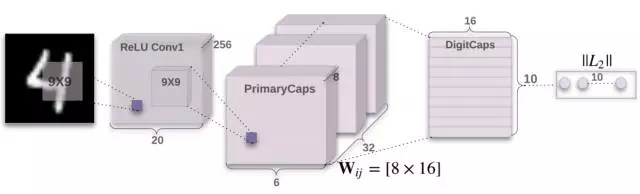
\includegraphics[scale=0.5]{CapsNet.png}
	\caption{CapsNet 网络}
	\label{fig:2}
\end{figure}
第一个卷积层使用了 256 个 $9\times9$ 卷积核,步幅为 1,且使用了 ReLU 激活函数。该卷积操作应该没有使用 Padding,输出的张量才能是 $20\times20\times256$。此外,CapsNet 的卷积核感受野使用的是 $9\times9$,相比于其它 $3\times3$ 或 $5\times5$ 的要大一些,这个能是因为较大的感受野在 CNN 层次较少的情况下能感受的信息越多。这两层间的权值数量应该为 $9\times9\times256+256=20992$。

随后,第二个卷积层开始作为 Capsule 层的输入而构建相应的张量结构。我们可以从上图看出第二层卷积操作后生成的张量维度为 $6\times6\times8\times32$,那么我们该如何理解这个张量呢?云梦居客在知乎上给出了一个十分形象且有意思的解释,如前面章节所述,如果我们先考虑 32 个(32 channel)$9\times9$ 的卷积核在步幅为 2 的情况下做卷积,那么实际上得到的是传统的 $6\times6\times32$ 的张量,即等价于 $6\times6\times1\time32$。
\begin{figure}[H]
	\centering
	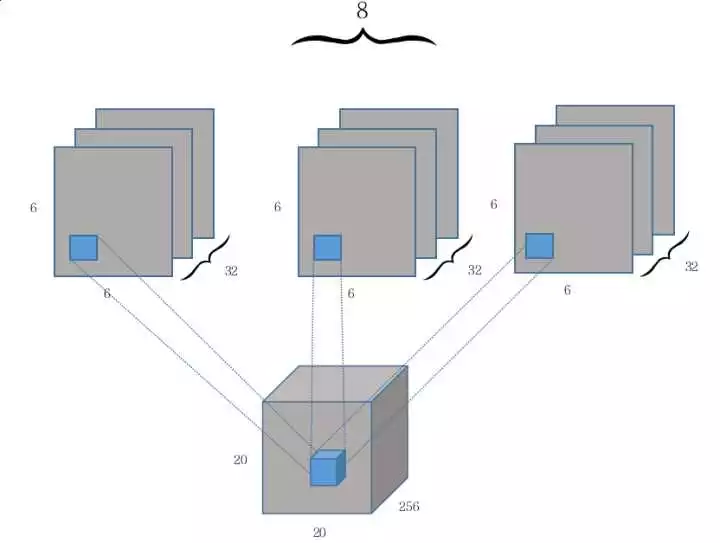
\includegraphics[scale=0.5]{CapsNet_OP.png}
	\caption{CapsNet 操作}
	\label{fig:3}
\end{figure}


因为传统卷积操作每次计算的输出都是一个标量,而 PrimaryCaps 的输出需要是一个长度为 8 的向量,因此传统卷积下的三维输出张量 $6\times6\times1\times32$ 就需要变化为四维输出张量 $6\times6\times8\times32$。如下所示,其实我们可以将第二个卷积层看作对维度为 $20\times20\times256$ 的输入张量执行 8 次不同权重的 Conv2d 操作,每次 Conv2d 都执行带 32 个 $9\times9$ 卷积核、步幅为 2 的卷积操作。
由于每次卷积操作都会产生一个 $6\times6\times1\times32$ 的张量,一共会产生 8 个类似的张量,那么将这 8 个张量(即 Capsule 输入向量的 8 个分量)在第三个维度上合并在一起就成了 $6\times6\times8\times32$。从上可知 PrimaryCaps 就相当于一个深度为 32 的普通卷积层,只不过每一层由以前的标量值变成了长度为 8 的向量。

此外,结合 Hinton 等人给出的 Capsule 定义,它就相当于一组常见的神经元,这些神经元封装在一起形成了新的单元。在本论文讨论的 CapsNet 架构中,我们将 8 个卷积单元封装在一起成为了一个新的 Caosule 单元。PrimaryCaps 层的卷积计算都没有使用 ReLU 等激活函数,它们以向量的方式预备输入到下一层 Capsule 单元中。

PrimaryCaps 每一个向量的分量层级是共享卷积权重的,即获取 $6\times6$ 张量的卷积核权重为相同的 $9\times9$ 个。这样该卷积层的参数数量为 $9\times9\times256\times8\times32+8\times32=5308672$,其中第二部分 $8\times32$ 为偏置项参数数量。

第三层 DigitCaps 在第二层输出的向量基础上进行传播与 Routing 更新。第二层共输出 $6\times6\times32=1152$ 个向量,每一个向量的维度为 8,即第 i 层共有 1152 个 Capsule 单元。而第三层 j 有 10 个标准的 Capsule 单元,每个 Capsule 的输出向量有 16 个元素。前一层的 Capsule 单元数是 1152 个,那么 $w_{ij}$ 将有 $1152\times10$ 个,且每一个 $w_{ij}$ 的维度为 $8\times16$。当 $u_i$ 与对应的 $w_{ij}$ 相乘得到预测向量后,我们会有 $1152\times10$ 个耦合系数 $c_{ij}$,对应加权求和后会得到 10 个 $16\times1$ 的输入向量。将该输入向量输入到「squashing」非线性函数中求得最终的输出向量 $v_j$,其中 $v_j$ 的长度就表示识别为某个类别的概率。

DigitCaps 层与 PrimaryCaps 层之间的参数包含两类,即 $W_{ij}$ 和 $c_{ij}$。所有 $W_{ij}$ 的参数数量应该是 $6\times6\times32\times10\times8\times16=1474560$,$c_{ij}$ 的参数数量为 $6\times6\times32\times10\times16=184320$,此外还应该有 $2\times1152\times10=23040$ 个偏置项参数,不过原论文并没有明确指出这些偏置项。最后小编计算出该三层 CapsNet 一共有 5537024 个参数,这并不包括后面的全连接重构网络参数。
\section{损失函数和最优化}
前面我们已经了解 DigitCaps 层输出向量的长度即某个类别的概率,那么我们该如何构建损失函数,并根据该损失函数迭代地更新整个网络?前面我们耦合系数 $c_{ij}$ 是通过一致性 Routing 进行更新的,他并不需要根据损失函数更新,但整个网络其它的卷积参数和 Capsule 内的 $W_{ij}$ 都需要根据损失函数进行更新。一般我们就可以对损失函数直接使用标准的反向传播更新这些参数,而在原论文中,作者采用了 SVM 中常用的 Margin loss,该损失函数的表达式为:
\begin{equation}
	L_c = T_c\max(0,m^{+}-\|\mathbf{v}_c\|)^2+\lambda(1-T_c)\max(0,\|\mathbf{v}_c\|-m^{-1})^2
\end{equation}
其中 c 是分类类别,$T_c$ 为分类的指示函数(c 存在为 1,c 不存在为 0),$m^{+}$ 为上边界,$m^{-}$ 为下边界。此外,$v_c$ 的模即向量的 L2 距离。

因为实例化向量的长度来表示 Capsule 要表征的实体是否存在,所以当且仅当图片里出现属于类别 k 的手写数字时,我们希望类别 k 的最顶层 Capsule 的输出向量长度很大(在本论文 CapsNet 中为 DigitCaps 层的输出)。为了允许一张图里有多个数字,我们对每一个表征数字 k 的 Capsule 分别给出单独的 Margin loss。

构建完损失函数,我们就能愉快地使用反向传播了。
\section{重构和表征}
重构即我们希望利用预测的类别重新构建出该类别代表的实际图像,例如我们前面部分的模型预测出该图片属于一个类别,然后后面重构网络会将该预测的类别信息重新构建成一张图片。

前面我们假设过 Capsule 的向量可以表征一个实例,那么如果我们将一个向量投入到后面的重构网络中,它应该能重构出一个完整的图像。因此,Hinton 等人使用额外的重构损失(reconstruction loss)来促进 DigitCaps 层对输入数字图片进行编码。下图展示了整个重构网络的的架构:
\begin{figure}[H]
	\centering 
	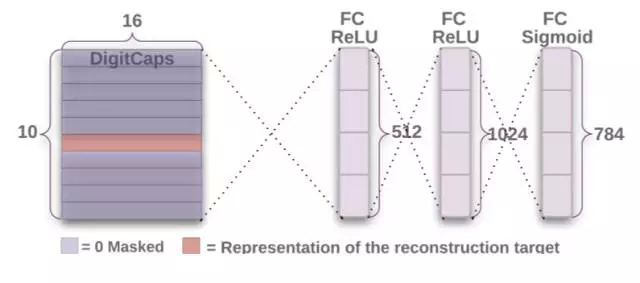
\includegraphics[scale=0.5]{CapsNet_recon.png}
	\caption{重构}
	\label{fig:4}
\end{figure}
我们在训练期间,除了特定的 Capsule 输出向量,我们需要蒙住其它所有的输出向量。然后,使用该输出向量重构手写数字图像。DigitCaps 层的输出向量被馈送至包含 3 个全连接层的解码器中,并以上图所示的方式构建。这一过程的损失函数通过计算 FC Sigmoid 层的输出像素点与原始图像像素点间的欧几里德距离而构建。Hinton 等人还按 0.0005 的比例缩小重构损失,以使它不会主导训练过程中的 Margin loss。

Capsule 输出向量的重构与表征除了能提升模型的准确度以外,还能提升模型的可解释性,因为我们能修正需要重构向量中的某个或某些分量而观察重构后的图像变化情况,这有助于我们理解 Capsule 层的输出结果。
